% Options for packages loaded elsewhere
\PassOptionsToPackage{unicode}{hyperref}
\PassOptionsToPackage{hyphens}{url}
\documentclass[
]{article}
\usepackage{xcolor}
\usepackage[margin=1in]{geometry}
\usepackage{amsmath,amssymb}
\setcounter{secnumdepth}{-\maxdimen} % remove section numbering
\usepackage{iftex}
\ifPDFTeX
  \usepackage[T1]{fontenc}
  \usepackage[utf8]{inputenc}
  \usepackage{textcomp} % provide euro and other symbols
\else % if luatex or xetex
  \usepackage{unicode-math} % this also loads fontspec
  \defaultfontfeatures{Scale=MatchLowercase}
  \defaultfontfeatures[\rmfamily]{Ligatures=TeX,Scale=1}
\fi
\usepackage{lmodern}
\ifPDFTeX\else
  % xetex/luatex font selection
\fi
% Use upquote if available, for straight quotes in verbatim environments
\IfFileExists{upquote.sty}{\usepackage{upquote}}{}
\IfFileExists{microtype.sty}{% use microtype if available
  \usepackage[]{microtype}
  \UseMicrotypeSet[protrusion]{basicmath} % disable protrusion for tt fonts
}{}
\makeatletter
\@ifundefined{KOMAClassName}{% if non-KOMA class
  \IfFileExists{parskip.sty}{%
    \usepackage{parskip}
  }{% else
    \setlength{\parindent}{0pt}
    \setlength{\parskip}{6pt plus 2pt minus 1pt}}
}{% if KOMA class
  \KOMAoptions{parskip=half}}
\makeatother
\usepackage{graphicx}
\makeatletter
\newsavebox\pandoc@box
\newcommand*\pandocbounded[1]{% scales image to fit in text height/width
  \sbox\pandoc@box{#1}%
  \Gscale@div\@tempa{\textheight}{\dimexpr\ht\pandoc@box+\dp\pandoc@box\relax}%
  \Gscale@div\@tempb{\linewidth}{\wd\pandoc@box}%
  \ifdim\@tempb\p@<\@tempa\p@\let\@tempa\@tempb\fi% select the smaller of both
  \ifdim\@tempa\p@<\p@\scalebox{\@tempa}{\usebox\pandoc@box}%
  \else\usebox{\pandoc@box}%
  \fi%
}
% Set default figure placement to htbp
\def\fps@figure{htbp}
\makeatother
\setlength{\emergencystretch}{3em} % prevent overfull lines
\providecommand{\tightlist}{%
  \setlength{\itemsep}{0pt}\setlength{\parskip}{0pt}}
\usepackage{bookmark}
\IfFileExists{xurl.sty}{\usepackage{xurl}}{} % add URL line breaks if available
\urlstyle{same}
\hypersetup{
  pdftitle={COVID-19 Vaccine Distribution Analysis},
  pdfauthor={Zoli Smith},
  hidelinks,
  pdfcreator={LaTeX via pandoc}}

\title{COVID-19 Vaccine Distribution Analysis}
\author{Zoli Smith}
\date{04-16-2025}

\begin{document}
\maketitle

{
\setcounter{tocdepth}{2}
\tableofcontents
}
\section{Introduction}\label{introduction}

The dataset used in this analysis pertains to the distribution of Pfizer
COVID-19 vaccine allocations across various jurisdictions. The primary
objective of this analysis is to explore the vaccine allocation by
jurisdiction and assess the relationship between population size and
vaccine allocation. We will load the dataset, summarize key variables,
and create both a table and a figure to visualize the data.

\subsubsection{Summary Table}\label{summary-table}

A summary table of key variables, such as Pfizer vaccine allocation and
jurisdiction population.

\subsubsection{Summary Table}\label{summary-table-1}

\subsubsection{Table Description}\label{table-description}

Table 1 summarizes the vaccine allocation by jurisdiction, showing both
the first and second dose allocations. This table offers a quick
overview of the distribution of vaccines across jurisdictions.

\subsection{Figure: Vaccine Allocation by
Jurisdiction}\label{figure-vaccine-allocation-by-jurisdiction}

This stacked bar chart displays the total vaccine allocations across the
top 10 jurisdictions, with the first dose shown in blue and the second
dose in orange. The jurisdictions are ordered by total allocations, and
the y-axis represents the total number of doses allocated. The chart
provides a clear comparison of both the first and second dose
distributions across the jurisdictions.

\pandocbounded{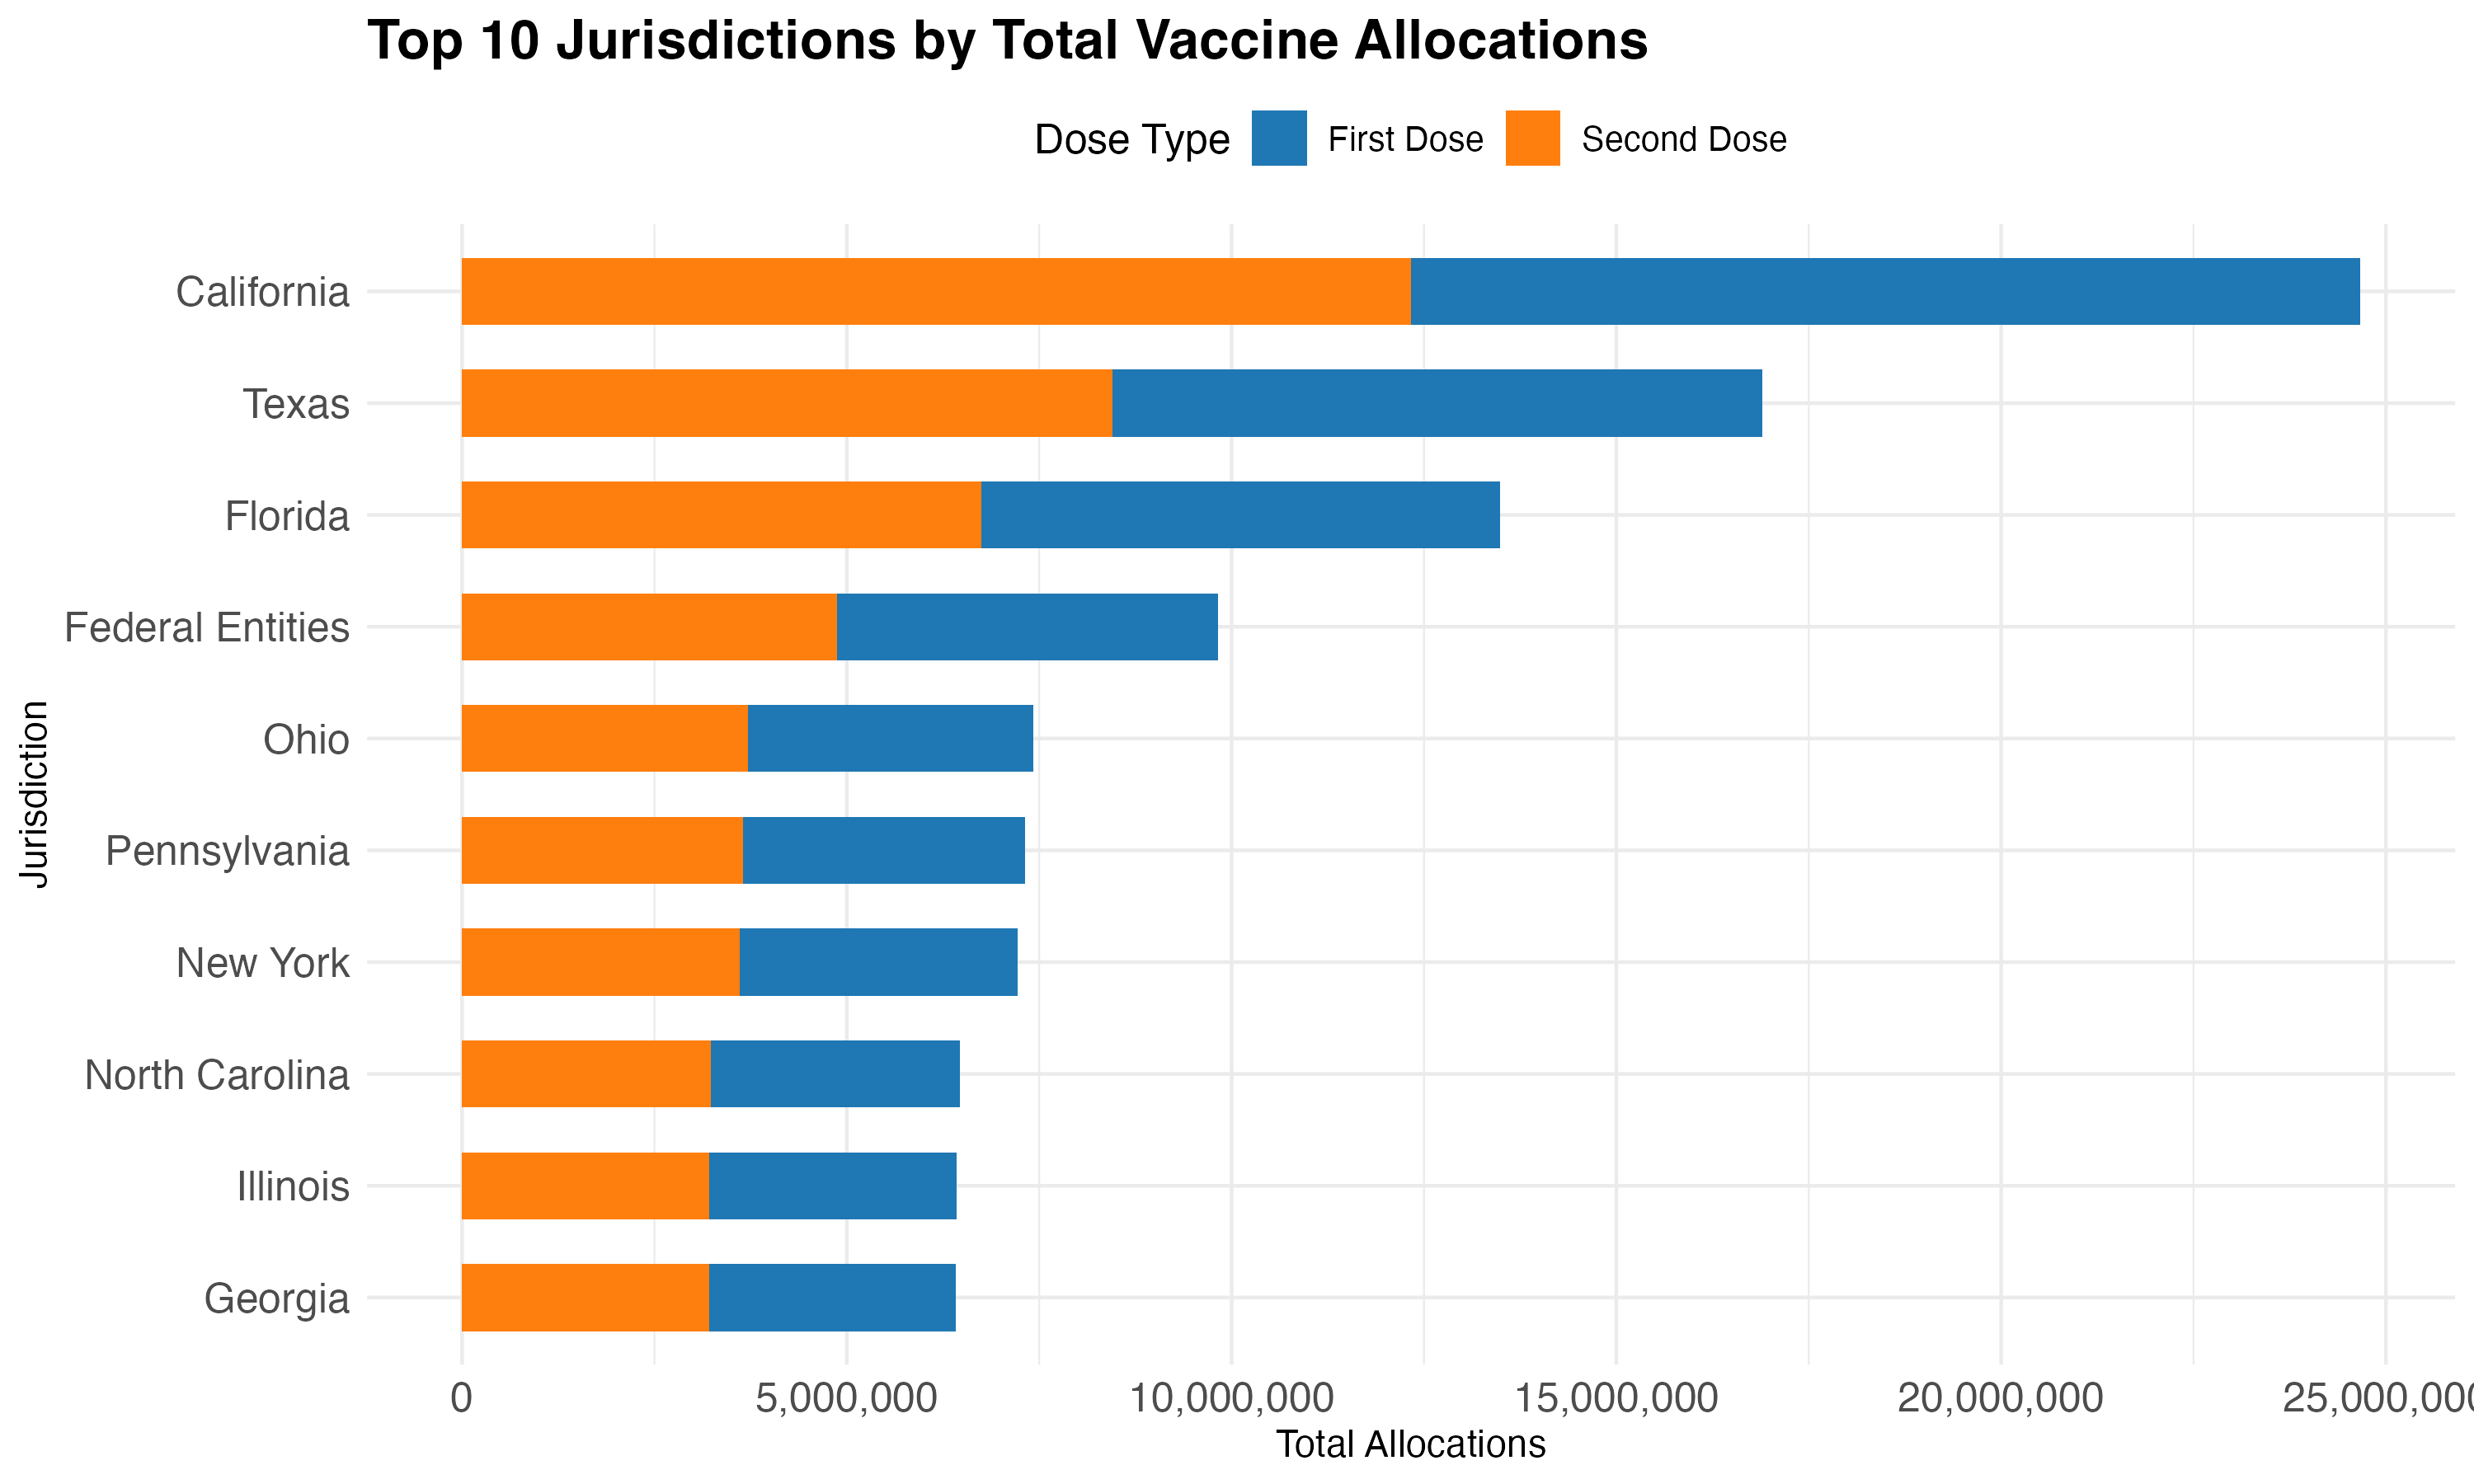
\includegraphics[keepaspectratio]{report/figures/required_figure.png}}

\end{document}
